\chapter{Implementation}


\section{Raspberry pi}
This section will describe the single board computer that is used for lane detection in this degree project. The chosen board is a Raspberry Pi 3 which is a credit card sized computer. The third generation of the raspberry has seen some major hardware updates compared to earlier versions. The one used in this project has the following specifications:



\begin{table}[H]
\centering
\caption{Raspberry Pi 3 Model B specifications}
\label{my-label}
\begin{tabular}{lllll}
 Model:	&Raspberry Pi 3 Model B  \\
 Operating system:	&Rasbian-Jessie  \\
 Processor:	&ARM Cortex-A53 1.2 GHz 64-bit quad-core  \\
 Hardware Ports:	&40 GPIO pins, 4 USB ports, HDMI port, Ethernet port,\\  &3.5 mm audio jack, Camera interface, Display interface,\\  &Micro SD card slot
\end{tabular}
\end{table}



The main computer in this project is the emc2 board and thus it would be prefered to utilize it for the lane detection as well. But due to no camera drivers available for the emc2 board it would be difficult to manage the image acquisition. A search for other hardware that is more suitable for the task was carried out and the raspberry pi was chosen due to that it is widely used in computer vision projects and its affordable pricepoint.

\subsection{Pi Camera}
The pi camera module has been chosen as image acquisition device for this project. The camera module has a five megapixel image sensor and a maximum resolution of 2952 x 1944 pixels. This camera was chosen due the fact that it is made specifically for the raspberry pi and is very easy to use. The one used has a wideangel lens which maybe is not optimal??






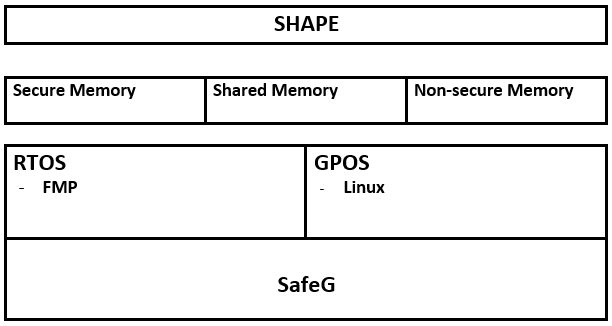
\includepdf[scale=0.8,pages=1,pagecommand=\section{System architecture}]{./img/architecture.pdf}

\section{Lane detection algorithm}


This chapter will describe the algorithms used for lane detection that have been implemented on the demonstator of this project. 

The algorithm that has been implemented on the demonstator so far consist of the following steps:

The lane detection process starts with grabbing a frame from the pi camera and applying a few preprocessing steps to the image. 

The first step is to crop the image to only contain the region of interest (ROI). This is a camera setting that can be predefined so that the camera only grabs the ROI and thus not need to crop it after the frame is grabbed.


Following step is to convert the image to gray scale to prepare it for nextcoming operations. 



\begin{figure}[H]
  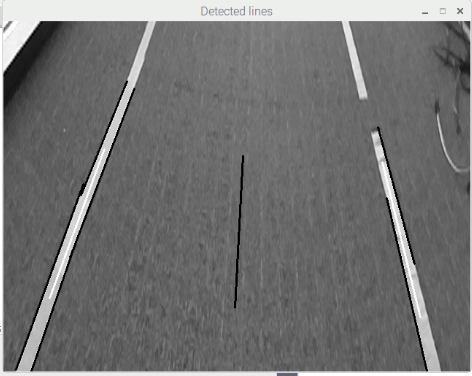
\includegraphics[scale=0.7]{./img/gray.png}
  \centering
  \caption{Input image converted to grayscale}
  \label{fig:Input image converted to grayscale}
\end{figure}


The grayscale image is the input to the canny edge detection function. As described in the state of the art section the output of the canny function is a thresholded image where all the pixels that are part of edges are set to white and all pixels that are not part of edges are set black.

\begin{figure}[H]
  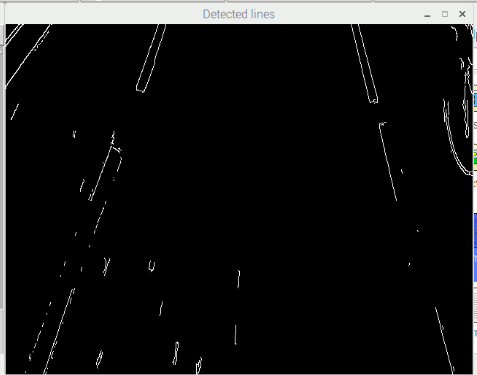
\includegraphics[scale=0.7]{./img/edges.png}
  \centering
  \caption{Tresholded image using canny filter}
  \label{fig:Tresholded image using canny filter}
\end{figure}

This tresholded image is used as an input to the hough transform function that is used for line detection. The function works by::(FÖRKLARING HOUGH)


\begin{figure}[H]
  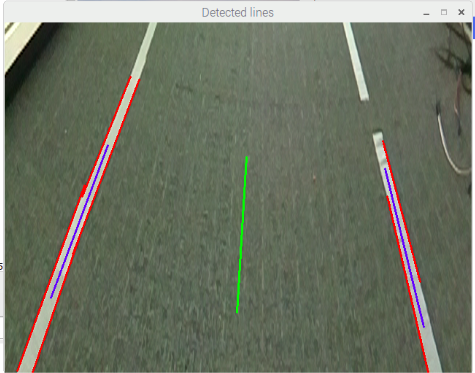
\includegraphics[scale=0.7]{./img/detected_lines.png}
  \centering
  \caption{Detected lines}
  \label{fig:Detected lines}
\end{figure}


Now the lines are detected and the data  output from the houghlines function need to be handled in some way. 
The algotihm created works by splititng the image into two halves and making the asumption that we have one lane in each of the two halves. By measuring the distance to the line from the center of the image, the error is calculated as $error = xtot - xmid$





\section{Lateral control}
So far all of these steps are all done on the Raspberry Pi thanks to its easy camera implementation and that it supports OpenCV. The error is then sent to the EMC2 board where the lateral control is done using the error from the RPi. A PID controller for the steering servo is developed using z transform.
